\chapter{剑指150}
开始于2023年3月1日\\高昆轮
\section{第一章 函数极限连续}
\subsection{考点1 常用函数及常用曲线p4}
\subsubsection{函数的概念及一些常用函数}
\begin{enumerate}
    \item 绝对值函数\\
    y=|x|在x=0处连续,但是是不可导的(左导数不等于右导数)\par
        \begin{equation*}
        y=|x|=
        \scaleleftright[6pt]{\biggl\{}{
        \begin{aligned}
        & x,\ x\ge 0 \\
        & -x,\ x<0
        \end{aligned}
        }{.}
        \end{equation*}
    \pmb{重要公式}$|a_1 \pm a_2 \pm... \pm a_n|\le|a_1|+|a_2|+...+|a_n|$

    \item 最值函数\\
    $U=max\{f(x),g(x)\}= \frac{f(x)+g(x)+|f(x)-g(x)|}{2}$\\
    $V=min\{f(x),g(x)\}= \frac{f(x)+g(x)-|f(x)-g(x)|}{2}$\\
    $U+V=f(x)+g(x),U-V=|f(x)-g(x)|,U \cdot V=f(x)g(x)$

    \item 符号函数\\
    对任何$x$,都有$\sqrt{x^2}=|x|=xsgn(x)$\par
    \begin{equation*}
        y=\text{sgn}\ x=
        \scaleleftright[6pt]{\biggl\{}{
            \begin{aligned}
                & 1,\ x>0 \\
                & 0,\ x=0 \\
                & -1,\ x<0
            \end{aligned}
            }{.}
        \end{equation*}
    
    \item 取整函数\\
    $[x+n]=[x]+n,其中n是整数,x-1<[x]\le x $
    
    \item 幂指函数\\
    $u(x)^{v(x)}=e^{v(x)lnu(x)}$
    
    \item 狄利克雷函数
    {
        % \begin{equation}
        $D(x)=\left\{
            \begin{array}{cl}
                1,&x\in Q\\
                0,&x\in Q^C\\
            \end{array}
            \right.$
        % \end{equation}
    }
\end{enumerate}

\subsection{反函数、复合函数及初等函数}
\begin{enumerate}
    \item 反函数
    \begin{enumerate}
        \item $y=\sin x$的反函数\\
        当$0\le x\le \frac{\pi}{2}$时,$x=\arcsin y,y\in [0,1]$\\
        当$\frac{\pi}{2}\le x\le \frac{3\pi}{2}$时,$x=\pi -\arcsin y,y\in [-1,1)$\\
        当$\frac{3\pi}{2}\le x\le 2\pi$时,$x=2\pi +\arcsin y,y\in (-1,0]$
    \end{enumerate}
    \item 复合函数
    \item 初等函数
    \begin{enumerate}
        \item 反对幂三指
        \item 幂指函数是初等函数
        \item 三角函数
            \begin{enumerate}
            \item 正弦函数和余弦函数\par
            正弦函数$ y=\sin x $, 余弦函数$ y=\cos x $.
            \item 正切函数和余切函数\par
            正切函数$ y=\tan x $, 余切函数$ y=\cot x $.\par
            \begin{figure}[H]
            \centering
            \begin{subfigure}{.475\linewidth}
            \centering
            \begin{tikzpicture}[
            ]
            \begin{axis}[
            width=\linewidth,
            axis lines=middle,
            xmin=-4.3,
            xmax=4.3,
            ymin=-4.5,
            ymax=4.5,
            xlabel=$ x $,
            ylabel=$ y $,
            xlabel=$ x $,
            xlabel style={below},
            ylabel=$ y $,
            ylabel style={left},
            xtick={-pi/2,pi/2},
            xticklabels={$ -\frac{\pi}{2} $,$ \frac{\pi}{2} $},
            xticklabel style={left,yshift=-0.5em},
            ytick={1},
            yticklabels={$ 1 $},
            extra y ticks={-1},
            extra y tick labels={$ -1 $},
            extra y tick style={tick label style={right,yshift=-1em}},
            ]
            \addplot [black,samples=1000]{tan(deg(x))};
            \end{axis}
            \end{tikzpicture}
            \caption{正切函数图像}
            \end{subfigure}
            \hspace{.1em}
            \begin{subfigure}{.475\linewidth}
            \centering
            \begin{tikzpicture}[
            ]
            \begin{axis}[
            width=\linewidth,
            axis lines=middle,
            xmin=-4.3,
            xmax=4.3,
            ymin=-4.5,
            ymax=4.5,
            xlabel=$ x $,
            xlabel style={below},
            ylabel=$ y $,
            ylabel style={left},
            xtick={-pi/2,pi/2},
            xticklabels={$ -\frac{\pi}{2} $,$ \frac{\pi}{2} $},
            xticklabel style={left,yshift=-0.5em},
            ytick={1},
            yticklabels={$ 1 $},
            extra y ticks={-1},
            extra y tick labels={$ -1 $},
            extra y tick style={tick label style={right,yshift=-1em}},
            ]
            \addplot [black,samples=1000]{1/tan(deg(x))};
            \end{axis}
            \end{tikzpicture}
            \caption{余切函数图像}
            \end{subfigure}
            \end{figure}
            \item 正割函数和余割函数\par
            正割函数$ y=\sec x $, 余割函数$ y=\csc x $.
            \begin{figure}[H]
            \centering
            \begin{subfigure}{.475\linewidth}
            \centering
            \begin{tikzpicture}[
            ]
            \begin{axis}[
            width=\linewidth,
            axis lines=middle,
            xmin=-4.3,
            xmax=4.3,
            ymin=-4.5,
            ymax=4.5,
            xlabel=$ x $,
            ylabel=$ y $,
            xtick={-pi/2,pi/2},
            xticklabels={$ -\frac{\pi}{2} $,$ \frac{\pi}{2} $},
            xticklabel style={left,yshift=-0.5em},
            ytick={-1,1},
            yticklabels={$ -1 $,$ 1 $},
            yticklabel style={below,xshift=-1em,yshift=0.4em},
            ]
            \addplot [black,samples=1000]{1/cos(deg(x))};
            \end{axis}
            \end{tikzpicture}
            \caption{正割函数图像}
            \end{subfigure}
            \begin{subfigure}{.475\linewidth}
            \begin{tikzpicture}[
            ]
            \begin{axis}[
            width=\linewidth,
            axis lines=middle,
            xmin=-4.3,
            xmax=4.3,
            ymin=-4.5,
            ymax=4.5,
            xlabel=$ x $,
            ylabel=$ y $,
            ylabel style={left},
            xtick={pi/2},
            xticklabels={$ \frac{\pi}{2} $},
            extra x ticks={-pi/2},
            extra x tick labels={$ -\frac{\pi}{2} $},
            extra x tick style={tick label style={above}},
            ytick={1},
            yticklabels={$ 1 $},
            extra y ticks={-1},
            extra y tick labels={$ -1 $},
            extra y tick style={tick label style={right,yshift=-0.5em}},
            ]
            \addplot [black,samples=1000]{1/sin(deg(x))};
            \end{axis}
            \end{tikzpicture}
            \caption{余割函数图像}
            \end{subfigure}
            \end{figure}
            \end{enumerate}
        \item 反三角函数
            \begin{enumerate}
            \item 反正弦函数和反余弦函数\par
            反正弦函数$ y=\arcsin x $, 反余弦函数$ y=\arccos x $.
            \begin{figure}[H]
            \centering
            \begin{subfigure}{.475\linewidth}
            \centering
            \begin{tikzpicture}[
            ]
            \begin{axis}[
            width=\linewidth,
            axis lines=middle,
            domain=-1:1,
            xmin=-2,
            xmax=2,
            ymin=-2,
            ymax=2,
            xlabel=$ x $,
            ylabel=$ y $,
            xtick={-1,1},
            ytick={-pi/2,pi/2},
            yticklabels={$ -\frac{\pi}{2} $, $ \frac{\pi}{2} $},
            ]
            \addplot [black,samples=1000]{asin(x)/180*pi};
            \end{axis}
            \end{tikzpicture}
            \caption{反正弦函数图像}
            \end{subfigure}
            \begin{subfigure}{.475\linewidth}
            \begin{tikzpicture}[
            ]
            \begin{axis}[
            width=\linewidth,
            axis lines=middle,
            domain=-1:1,
            xmin=-2,
            xmax=2,
            ymin=-0.5,
            ymax=4,
            xlabel=$ x $,
            ylabel=$ y $,
            ytick={pi/2,pi},
            yticklabels={$ \frac{\pi}{2} $, $ \pi $},
            xtick={-1,1},
            xticklabels={$ -1 $,$ 1 $},
            ]
            \addplot [black,samples=1000]{acos(x)/180*pi};
            \end{axis}
            \end{tikzpicture}
            \caption{反余弦函数图像}
            \end{subfigure}
            \end{figure}
            \item 反正切函数和反余切函数\par
            反正切函数$ y=\arctan x $, 反余切函数$ y=\arccot x $
            \begin{figure}[H]
            \centering
            \begin{subfigure}{.475\linewidth}
            \centering
            \begin{tikzpicture}[
            ]
            \begin{axis}[
            width=\linewidth,
            axis lines=middle,
            xmin=-2,
            xmax=2,
            ymin=-2,
            ymax=2,
            xlabel=$ x $,
            ylabel=$ y $,
            xtick={\empty},
            ytick={-pi/2,pi/2},
            yticklabels={$ -\frac{\pi}{2} $, $ \frac{\pi}{2} $},
            ]
            \addplot [black,samples=1000]{atan(x)/180*pi};
            \end{axis}
            \end{tikzpicture}
            \caption{反正切函数图像}
            \end{subfigure}
            \begin{subfigure}{.475\linewidth}
            \begin{tikzpicture}[
            ]
            \begin{axis}[
            width=\linewidth,
            axis lines=middle,
            xmin=-2,
            xmax=2,
            ymin=-0.5,
            ymax=4,
            xlabel=$ x $,
            ylabel=$ y $,
            ytick={pi/2,pi},
            yticklabels={$ \frac{\pi}{2} $, $ \pi $},
            xtick={\empty},
            ]
            \addplot [black,samples=1000]{(pi/2)-(atan(x))/180*pi};
            \end{axis}
            \end{tikzpicture}
            \caption{反余切函数图像}
            \end{subfigure}
            \end{figure}
            \end{enumerate}
    \end{enumerate}


\end{enumerate}

\subsection{函数表达式的求解}

\begin{enumerate}
    \item 一般借助微分方程(第八章)求解
    \item 注意$\lim \limits_{x\to x_0}f(x),f'(x_0),\int_{a}^{b}f(x)dx$等都是一个数
    \item 抓大头\\
    重要公式$\lim \limits_{n\to \infty}\sqrt{a_1^n+a_2^n+...+a_m^n}=max\{a_1,a_2,...,a_m\}$\\
    考点12例六

\end{enumerate}

\subsection{常用曲线(这些曲线在以后会经常碰到)}

\begin{enumerate}
    \item 笛卡尔心形线\\
    $x^2+y^2=a(\sqrt[]{x^2+y^2}-x)$或$r=a(1-\cos \theta)$(桃屁股朝右)\\
    $x^2+y^2=a(\sqrt[]{x^2+y^2}+x)$或$r=a(1+\cos \theta)$(桃屁股朝左)\\
    与$x$轴交点$O,\mp 2a$,与$y$轴交点$\pm a$\par
    $ r=a(1-\cos \theta)(a>0) $
    \begin{figure}[H]
        \centering
        \begin{tikzpicture}[
        >=stealth,
        ]
        \draw[->] (0,0)node[left]{$ 0 $} to (1,0)node[right]{$ x $};
        \draw[domain=0:360,samples=1000,scale=.7] plot (\x:{2*(1-cos(\x))});
        \end{tikzpicture}
        \caption{心形线}
    \end{figure}

    \item 玫瑰线\par
    $ r=a\sin 3\theta (a>0) $
    \begin{figure}[H]
        \centering
        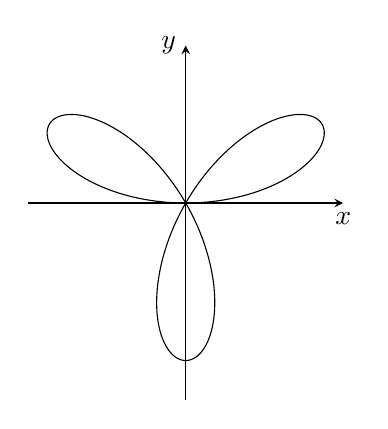
\begin{tikzpicture}[
        >=stealth,
        ]
        \draw[->] (-2,0) to (2,0)node[below]{$ x $};
        \draw[->] (0,-2.5) to (0,2)node[left]{$ y $};
        \draw[domain=0:360,samples=1000,scale=1] plot (\x:{2*sin(3*\x)});
        \end{tikzpicture}
        \caption{玫瑰线}
    \end{figure}
    
    \item 阿基米德螺线\par
    $ r=a\theta (a>0,\theta \ge 0) $
    \begin{figure}[H]
        \centering
        \begin{tikzpicture}[
        >=stealth,
        ]
        \draw[->] (0,0)node[left]{$ 0 $} to (3,0)node[below]{$ x $};
        \draw[domain=0:360,samples=1000,scale=.2] plot (\x:{2*(\x/180*pi)});
        \end{tikzpicture}
        \caption{阿基米德螺线}
    \end{figure}

    \item 伯努利双纽线\par
    $ r^{2}=a^{2}\cos 2\theta(a>0) $一二三四象限\\
    $ r^{2}=a^{2}\sin 2\theta(a>0) $一三象限.
    \begin{figure}[H]
        \centering
        \begin{subfigure}{.475\linewidth}
        \centering
        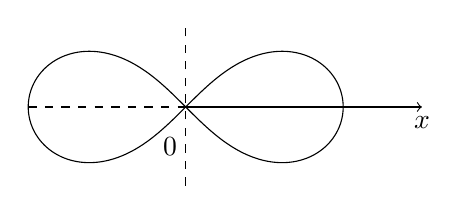
\begin{tikzpicture}
        \draw[->] (0,0) to (3,0)node[below]{$ x $};
        \node at (-.2,-.5){$ 0 $};
        \draw[dashed] (0,-1) to (0,1);
        \draw[dashed] (-2,0) to (0,0);
        \draw[domain=0:45,samples=1000] plot (\x:{sqrt(4*cos(2*\x))});
        \draw[domain=135:225,samples=1000] plot (\x:{sqrt(4*cos(2*\x))});
        \draw[domain=315:360,samples=1000] plot (\x:{sqrt(4*cos(2*\x))});
        \end{tikzpicture}
        \caption{$ r^{2}=a^{2}\cos 2\theta $}
        \end{subfigure}
        \hfill
        \begin{subfigure}{.475\linewidth}
        \centering
        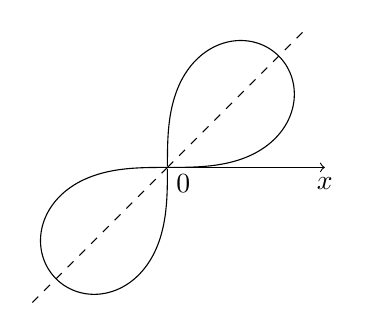
\begin{tikzpicture}
        \draw[->] (0,0) to (2,0)node[below]{$ x $};
        \node at (.2,-.2){$ 0 $};
        \draw[domain=0:90,samples=1000,] plot (\x:{sqrt(4*sin(2*\x))});
        \draw[domain=180:270,samples=1000,] plot (\x:{sqrt(4*sin(2*\x))});
        \draw[dashed] (0,0) to (45:2.5);
        \draw[dashed] (0,0) to (225:2.5);
        \end{tikzpicture}
        \caption{$ r^{2}=a^{2}\sin 2\theta $}
        \end{subfigure}
        \caption{伯努利双纽线}
    \end{figure}

    \item 摆线\par
    \begin{equation*}
        \scaleleftright[6pt]{\biggl\{}{
        \begin{aligned}
        & x=a(\theta-\sin \theta) \\
        & y=a(1-\cos \theta)
        \end{aligned}
        }{.}
    \end{equation*}
    \begin{figure}[H]
        \centering
        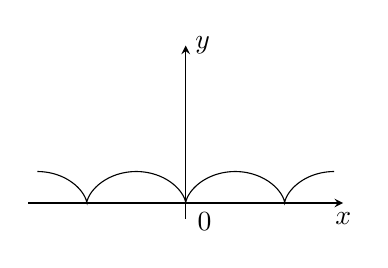
\begin{tikzpicture}[
        >=stealth,
        scale=2,
        ]
        \draw[->] (-1,0) to (1,0)node[below]{$ x $};
        \draw[->] (0,-.1) to (0,1)node[right]{$ y $};
        \node at (.12,-.12){$ 0 $};
        \draw[domain=-540:540][samples=1000] plot({(\x/180*pi-sin(\x))*0.1},{(1-cos(\x))*0.1});
        \end{tikzpicture}
        \caption{摆线}
    \end{figure}

    \item 星形线\par
    \begin{equation*}
        \scaleleftright[6pt]{\biggl\{}{
        \begin{aligned}
        & x=a\cos^{3}t \\
        & y=a\sin^{3}t
        \end{aligned}
        }{.}
    \end{equation*}
    \begin{figure}[H]
        \centering
        \begin{tikzpicture}[
        >=stealth,
        scale=2,
        ]
        \draw[->] (-1,0) to (1.2,0)node[below]{$ x $};
        \draw[->] (0,-1) to (0,1.2)node[right]{$ y $};
        \node at (.12,-.12){$ 0 $};
        \draw[domain=0:360][samples=1000] plot({(cos(\x))^3},{(sin(\x))^3});
        \end{tikzpicture}
        \caption{星形线}
    \end{figure}

    \item 笛卡尔叶形线\par
    {
        $x^3+y^3-3axy=0$或$\left\{ \begin{array}{cl}
            x=\frac{3at}{1+t^3},\\
            y=\frac{3at^2}{1+t^3}
        \end{array}\right.$
    }\\
    渐近线$y=x$和$x+y=-a$
\end{enumerate}


\section{考点2 函数的几种特性(特别要记忆对这些特性总结的结论)p11}

\subsubsection{有界性}

\begin{enumerate}
    \item 有界无界应在具体区间判断
    \item 有界无界的判定方法\begin{enumerate}
        \item 
    \end{enumerate}
\end{enumerate}

\subsubsection{单调性}

\subsubsection{奇偶性}

\subsubsection{周期性}

\section{考点3 极限的定义p14}

\section{考点4 极限的性质p19}

\section{考点5 无穷小与无穷大p20}

\section{考点6 极限的四则运算法则及两个重要极限p25}

\subsection{极限的四则运算法则}

\begin{enumerate}
    \item 若$\lim f(x)=A (\exists)$,$\lim g(x)=B (\exists)$
    \begin{enumerate}
        \item $\lim [f(x)\pm g(x)]=\lim f(x)\pm g(x)=A\pm B$
        \item $\lim [f(x)g(x)]=\lim f(x)\cdot g(x)=A \cdot B$
        \item $\lim \frac{f(x)}{g(x)}=\frac{\lim f(x)}{\lim g(x)}=\frac{A}{B}(B\ne 0)$
    \end{enumerate}
    \item 必须保证$\lim f(x)$和$\lim g(x)$都\pmb{存在},且运算项数为\pmb{有限项}
    \item 若$\lim f(x)$存在,$\lim g(x)$不存在,则$\lim [f(x)\pm g(x)]$必不存在
    \item 若$\lim f(x)$不存在,$\lim g(x)$不存在,则$\lim [f(x)\pm g(x)]$不一定不存在(可能存在)
    \item 若$\lim \frac{f(x)}{g(x)}=A$,且$\lim g(x)=0$,则$\lim f(x)=0$ \pmb{“母为0,推子为0”}
    \item 若$\lim \frac{f(x)}{g(x)}=A\ne 0$,且$\lim f(x)=0$,则$\lim g(x)=0$ \pmb{“子为0,推母为0”}
\end{enumerate}

\subsection{极限的四则运算法则的推广}

\begin{enumerate}
    \item \underline{在加减中存在极限的那部分}可以单独先算
    \item \underline{在乘除法中极限不为0的那部分}可以单独先算
\end{enumerate}

\subsection{两个重要极限}

\begin{enumerate}
    \item {$\lim \limits_{x\to 0}\frac{\sin x}{x}=1$\\ 该极限呈现$\frac{0}{0}$型未定式}
    \item {$\lim \limits_{x\to 0}(1+x)^{\frac{1}{x}}=e$\\ 该极限呈现$\frac{\infty}{\infty}$型未定式}
\end{enumerate}

\section{考点7 等价代换p29}

\subsubsection{常用的等价无穷小}

\begin{multicols}{4}
\begin{itemize}
    \item $ \sin x\sim x $
    \item $ \arcsin x\sim x $
    \item $ \ln (1+x)\sim x $
    \item $ \alpha^{x}-1\sim x\ln a $
    \item $ \tan x\sim x $
    \item $ \arctan x\sim x $
    \item $ e^{x}-1\sim x $
    \item $ (1+x)^{\alpha}-1\sim \alpha x $
    \item $ 1-\cos x\sim \frac{1}{2}x^{2} $
    \item $ 1-\cos^{\alpha} x\sim \frac{\alpha}{2}x^{2} $
    \end{itemize}
\end{multicols}

\subsubsection{等价无穷替换原则}

凡是在(\pmb{或处理后在})同一个$\lim$里表现为乘除运算的无穷小都可对其使用等价代换

对于$e^{f(x)}-e^{g(x)}$,往往采用\pmb{提公因子$e^{g(x)}$}的方式处理,即$e^{f(x)}-e^{g(x)}=e^{g(x)}[e^{f(x)-g(x)}-1]$

对$A-B$应当先观察是否有公因子,若有,则将其提出

\section{考点8 洛必达法则}

\section{考点9 泰勒公式(多项式的高次逼近)p35}

\subsection{泰勒公式}
% \newpage
\subsubsection{泰勒公式表}
\begin{multicols}{2}
    \begin{itemize}
    \item $ \sin x=x-\frac{x^{3}}{3!}+o(x^{3}) $
    \item $ e^{x}=1+x+\frac{x^{2}}{2!}+\frac{x^{3}}{3!}+o(x^{3}) $
    \item $ \arcsin x=x+\frac{x^{3}}{3!}+o(x^{3}) $
    \item $ \tan x=x+\frac{x^{3}}{3}+o(x^{3}) $
    \item $ \cos x=1-\frac{x^{2}}{2!}+\frac{x^{4}}{4!}+o(x^{4}) $
    \item $ ln(1+x)=x-\frac{x^{2}}{2}+\frac{x^{3}}{3}+o(x^{3}) $
    \item $ \arctan x=x-\frac{x^{3}}{3}+o(x^{3}) $
    \item $ (1+x)^{\alpha}=1+\alpha x+\frac{\alpha (\alpha -1)}{2!}x^{2}+\frac{\alpha (\alpha -1)(\alpha -2)}{3!}x^{3}+o(x^{3}) $
    \item $ ln(x+\sqrt{1+x^2})=x-\frac{1}{6}x^3+\frac{3}{40}x^5+o(x^3) $
    \end{itemize}
\end{multicols}

\begin{figure}
    \centering %表示居中
    % \includegraphics[height=0.5\paperheight]{./img/taylor-expansions.JPG}
\end{figure}


% \end{multicols}

\subsubsection{用泰勒公式求极限}
\begin{enumerate}
\item $ \frac{A}{B} $: 适用于``上下同阶''的原则 \par
如果分母(或者分子)是$ x $的$ k $此幂, 则应该把分子(或分母)展开到$ x $的$ k $次幂.
\item $ A-B $: 适用于幂次最低原则 \par
将$ A, B $分别展开到它们的系数不相等的$ x $的最低次幂为止.
\end{enumerate}

\section{考点10 幂指函数$u(x)^{v(x)}$的极限p38}

\section{考点11 已知极限反求参数及无穷小阶数的比较p40}

\section{考点12 数列的极限p43}

\section{考点13 函数的连续性与间断点p48}

\section{考点14 闭区间上连续函数的性质p53}

\chapter{一元函数微分学}

\section{考点15 导数定义}

\section{考点16 四则、复合函数、反函数及对数求导法则p62}

\section{考点17 高阶导数p65}

\section{考点18 隐函数及由参数方程所确定的函数的求导法则p67}

\section{考点19 分段函数及绝对值函数求导p70}

\section{考点20 导数的几何、物理意义及相关变化率p75}

\section{考点21 函数的微分p77}

\section{考点22 中值定理p80}

\section{考点23 单调性与极值、最值p91}

\section{考点24 凹凸性与拐点p99}

\section{考点25 渐近线、曲率p102}

\section{考点26 函数图形的描绘p105}

\section{考点27 证明函数或常数不等式p106}

\section{考点28 用导数讨论方程的根p109}

\chapter{一元函数积分学}

\section{考点29 原函数与不定积分的概念、积分公式p114}

\section{考点30 凑微分法求不定积分p117}

\section{考点31 换元法求不定积分p120}

\section{考点32 分布积分法求不定积分p121}

\section{考点33 有理函数的积分p124}

\section{考点34 定积分的定义及性质p125}

\section{考点35 定积分的计算方法及若干技巧p132}

\section{考点36 变限积分函数及其求导原理p140}

\section{考点37 变限积分函数的综合题p145}

\section{考点38 定积分不等式的证明p150}

\section{考点39 定积分与极限的综合题p154}

\section{考点40 反常积分p157}

\section{考点41 平面图形的面积p161}

\section{考点42 空间图形的体积p165}

\section{考点43 平面曲线的弧长p168}

\section{考点44 旋转曲面的侧面积p169}

\section{考点45 定积分的物理应用p170}

\chapter{向量代数与空间解析几何}

\section{考点46 向量及其运算p173}

\section{考点47 平面积空间直线p175}

\section{考点48 曲面及空间曲线p180}

\chapter{多元函数微分学}

\section{考点49 二元函数的极限及连续p185}

\section{考点50 偏导数p188}

\section{考点51 全微分p192}

\section{考点52 复合函数的偏导数与全微分p195}

\section{考点53 隐函数的偏导数及全微分p200}

\section{考点54 极值与最值p203}

\section{考点55 多元函数微分学的几何应用p209}

\section{考点56 方向导数与梯度p212}

\section{考点57 二元函数的二阶泰勒公式p214}

\chapter{多元函数积分学}

\section{考点58 二重积分概念与几何意义p217}

\section{考点59 直角坐标计算二重积分p221}

\section{考点60 极坐标计算二重积分p224}

\section{考点61 换序及换系p227}

\section{考点62 需分区域计算的几种情况p233}

\section{考点63 先一后二法(投影法)与先二后一法(截面法)p236}

\section{考点64 利用球面坐标计算三重积分p240}

\section{考点65 三重积分的性质及换序p241}

\section{考点66 第一类(平面、空间)曲线积分p242}

\section{考点67 第二类平面曲线积分p246}

\section{考点68 第一类曲面积分p253}

\section{考点69 第二类曲面积分p256}

\section{考点70 第二类空间曲线积分的计算p262}

\section{考点71 多元函数积分学的应用及场论初步p264}

\chapter{无穷级数}

\section{考点72 用定义和基本性质判断技术的敛散性p270}

\section{考点73 正项级数敛散性的判别方法p272}

\section{考点74 交错基数敛散性的判别方法p276}

\section{考点75 任意项基数敛散性的判别方法p278}

\section{考点76 收敛发散的证明题p281}

\section{考点77 幂级数的收敛半径及收敛域的求法p282}

\section{考点78 求一般函数项级数的收敛域p286}

\section{考点79 函数展开成幂级数p286}

\section{考点80 幂级数的和函数的求法p290}

\section{考点81 常数项级数的求和p295}

\section{考点82 傅立叶级数p297}

\chapter{常微分方程}

\section{考点83 微分方程的基本概念p301}

\begin{enumerate}
    \item 微分方程的通解与特解\\
        不含任意常数的解称为特解\\
        含独立任意常数个数与微分方程阶数相同的解称为微分方程的通解\\
        阶数与个数相同
    \item 线性与非线性微分方程\\
    看与y有关的次方是几次,若大于等于2次即为非线性

\end{enumerate}

\section{考点84 一阶微分方程p302}

\section{考点85 二阶可降阶的微分方程p307}

\section{考点86 常系数线性微分方程及欧拉方程p308}

\section{考点87 已知方程的解反求方程及进一步研究方程的解p312}

\section{考点88 通过变形改造建立微分方程并求解p318}

\section{考点89 微分方程的应用p323}

